\section{opttritri.cc File Reference}
\label{opttritri_8cc}\index{opttritri.cc@{opttritri.cc}}
{\tt \#include \char`\"{}opttritri.h\char`\"{}}\par
{\tt \#include \char`\"{}controls.h\char`\"{}}\par


Include dependency graph for opttritri.cc:\begin{figure}[H]
\begin{center}
\leavevmode
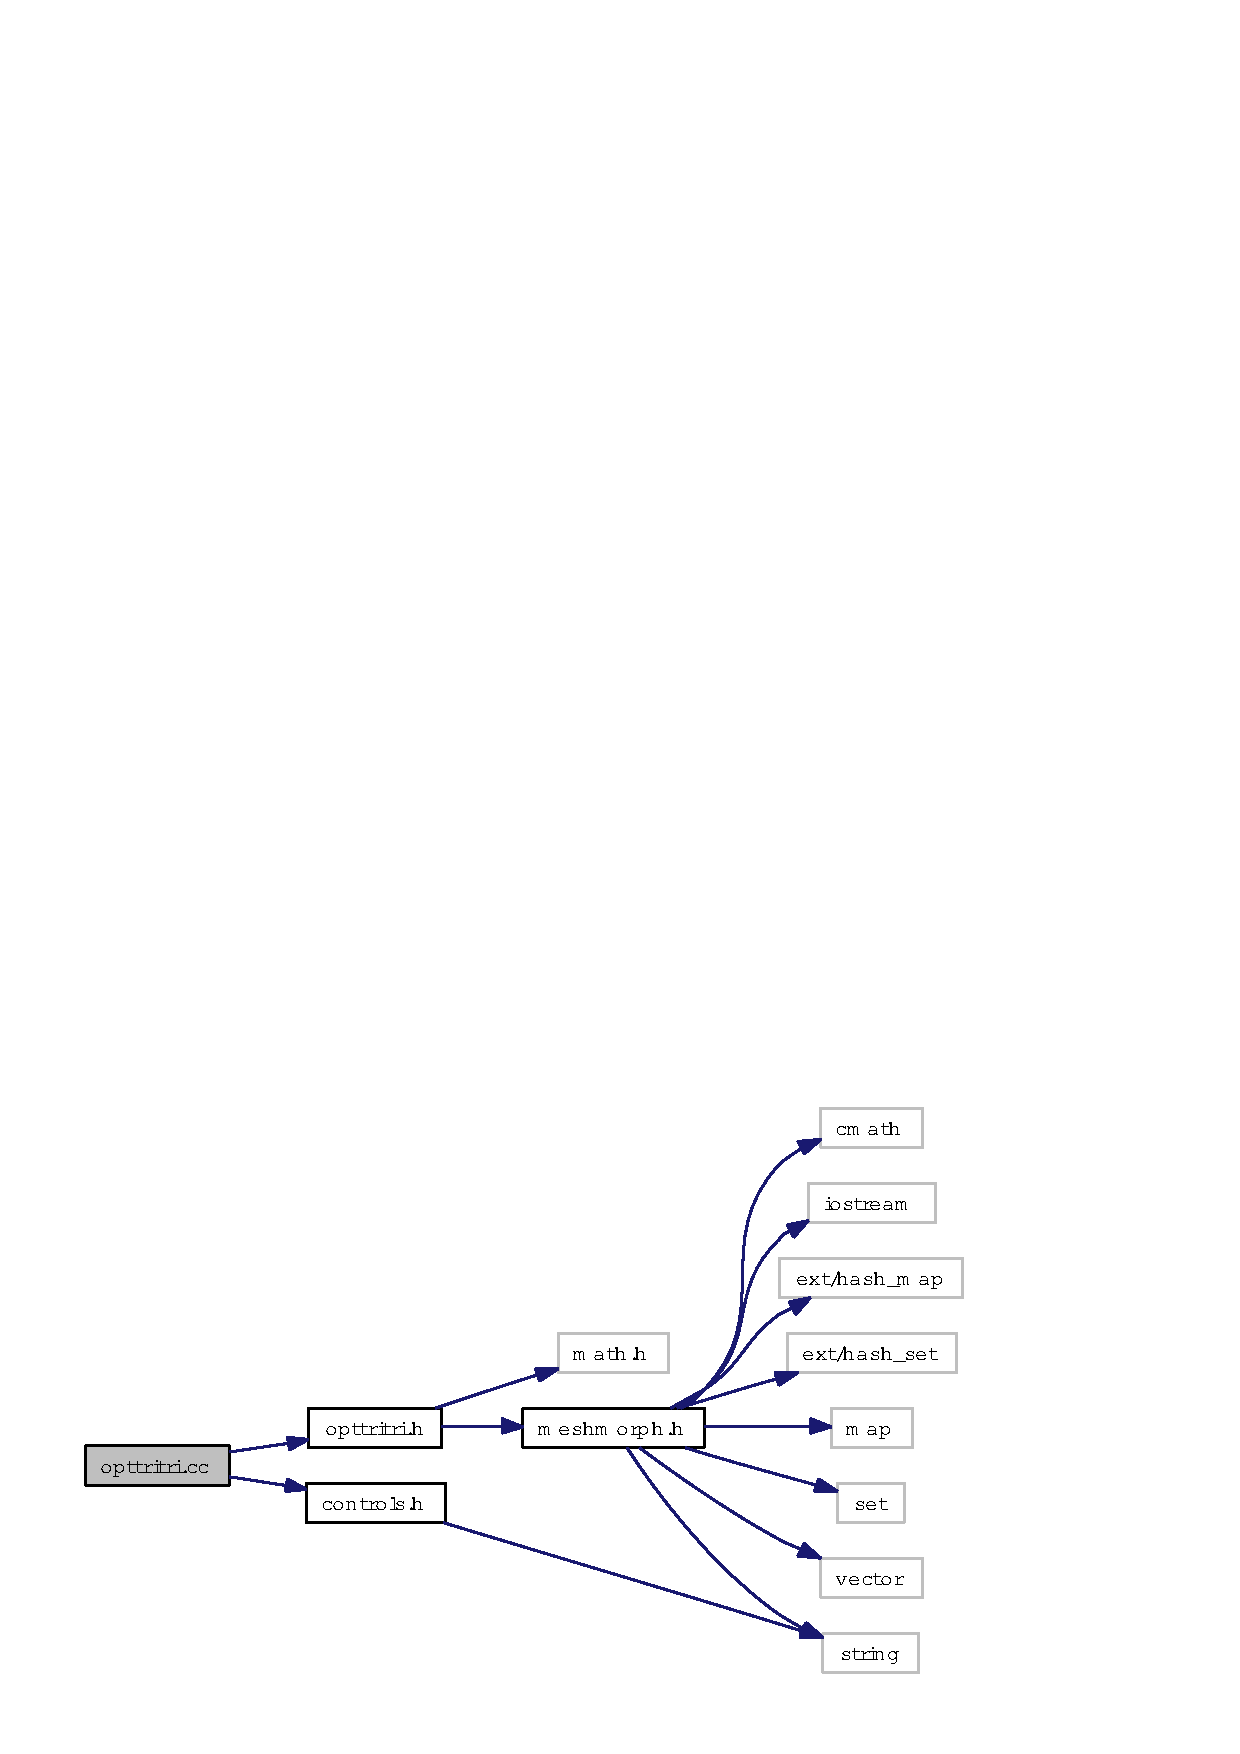
\includegraphics[width=233pt]{opttritri_8cc__incl}
\end{center}
\end{figure}
\subsection*{Functions}
\begin{CompactItemize}
\item 
int {\bf coplanar\_\-tri\_\-tri} ({\bf vector3} \&N, {\bf vector3} const $\ast$V0, {\bf vector3} const $\ast$V1, {\bf vector3} const $\ast$V2, {\bf vector3} const $\ast$U0, {\bf vector3} const $\ast$U1, {\bf vector3} const $\ast$U2)
\item 
int {\bf No\-Div\-Tri\-Tri\-Isect} ({\bf vector3} const $\ast$V0, {\bf vector3} const $\ast$V1, {\bf vector3} const $\ast$V2, {\bf vector3} const $\ast$U0, {\bf vector3} const $\ast$U1, {\bf vector3} const $\ast$U2)
\item 
int {\bf intersect\_\-triangle3} ({\bf vector3} const $\ast$orig, {\bf vector3} const $\ast$end, {\bf vector3} const $\ast$normal, {\bf vector3} const $\ast$vert0, {\bf vector3} const $\ast$vert1, {\bf vector3} const $\ast$vert2, {\bf result} \&r)
\end{CompactItemize}


\subsection{Function Documentation}
\index{opttritri.cc@{opttritri.cc}!coplanar_tri_tri@{coplanar\_\-tri\_\-tri}}
\index{coplanar_tri_tri@{coplanar\_\-tri\_\-tri}!opttritri.cc@{opttritri.cc}}
\subsubsection{\setlength{\rightskip}{0pt plus 5cm}int coplanar\_\-tri\_\-tri ({\bf vector3} \& {\em N}, {\bf vector3} const $\ast$ {\em V0}, {\bf vector3} const $\ast$ {\em V1}, {\bf vector3} const $\ast$ {\em V2}, {\bf vector3} const $\ast$ {\em U0}, {\bf vector3} const $\ast$ {\em U1}, {\bf vector3} const $\ast$ {\em U2})}\label{opttritri_8cc_7cc10013bc791c2bfab4bb52a1a2809e}


Determine whether two coplanar triangles intersect. \begin{Desc}
\item[Parameters:]
\begin{description}
\item[\mbox{$\leftarrow$} {\em N}]Not sure what this is. \item[\mbox{$\leftarrow$} {\em V0}]First vertex of first triangle. \item[\mbox{$\leftarrow$} {\em V1}]second vertex of first triangle. \item[\mbox{$\leftarrow$} {\em V2}]Third vertex of first triangle. \item[\mbox{$\leftarrow$} {\em U0}]First vertex of second triangle. \item[\mbox{$\leftarrow$} {\em U1}]second vertex of second triangle. \item[\mbox{$\leftarrow$} {\em U2}]Third vertex of second triangle. \end{description}
\end{Desc}
\begin{Desc}
\item[Returns:]1 if triangles intersect; 0 otherwise. \end{Desc}
\index{opttritri.cc@{opttritri.cc}!intersect_triangle3@{intersect\_\-triangle3}}
\index{intersect_triangle3@{intersect\_\-triangle3}!opttritri.cc@{opttritri.cc}}
\subsubsection{\setlength{\rightskip}{0pt plus 5cm}int intersect\_\-triangle3 ({\bf vector3} const $\ast$ {\em orig}, {\bf vector3} const $\ast$ {\em end}, {\bf vector3} const $\ast$ {\em normal}, {\bf vector3} const $\ast$ {\em vert0}, {\bf vector3} const $\ast$ {\em vert1}, {\bf vector3} const $\ast$ {\em vert2}, {\bf result} \& {\em r})}\label{opttritri_8cc_d7a9482aa12886f663ad07d306fe8ccb}


Determine if line segment and triangle intersect. \begin{Desc}
\item[Parameters:]
\begin{description}
\item[\mbox{$\leftarrow$} {\em orig}]One end of line segment. \item[\mbox{$\leftarrow$} {\em end}]Other end of line segment. \item[\mbox{$\leftarrow$} {\em normal}]Normal vector of triangle. \item[\mbox{$\leftarrow$} {\em vert0}]First vertex of triangle. \item[\mbox{$\leftarrow$} {\em vert1}]second vertex of triangle. \item[\mbox{$\leftarrow$} {\em vert2}]Third vertex of triangle. \item[\mbox{$\rightarrow$} {\em r}]Record whether line intersects triange along line segment; whether line intersects triangle; and whether line intersects edge of triangle. \end{description}
\end{Desc}
\begin{Desc}
\item[Returns:]1 if triangles intersect; 0 otherwise. \end{Desc}
\index{opttritri.cc@{opttritri.cc}!NoDivTriTriIsect@{NoDivTriTriIsect}}
\index{NoDivTriTriIsect@{NoDivTriTriIsect}!opttritri.cc@{opttritri.cc}}
\subsubsection{\setlength{\rightskip}{0pt plus 5cm}int No\-Div\-Tri\-Tri\-Isect ({\bf vector3} const $\ast$ {\em V0}, {\bf vector3} const $\ast$ {\em V1}, {\bf vector3} const $\ast$ {\em V2}, {\bf vector3} const $\ast$ {\em U0}, {\bf vector3} const $\ast$ {\em U1}, {\bf vector3} const $\ast$ {\em U2})}\label{opttritri_8cc_964292b46316fc46d2be9ca9570deb64}


Determine whether two triangles intersect. \begin{Desc}
\item[Parameters:]
\begin{description}
\item[\mbox{$\leftarrow$} {\em V0}]First vertex of first triangle. \item[\mbox{$\leftarrow$} {\em V1}]second vertex of first triangle. \item[\mbox{$\leftarrow$} {\em V2}]Third vertex of first triangle. \item[\mbox{$\leftarrow$} {\em U0}]First vertex of second triangle. \item[\mbox{$\leftarrow$} {\em U1}]second vertex of second triangle. \item[\mbox{$\leftarrow$} {\em U2}]Third vertex of second triangle. \end{description}
\end{Desc}
\begin{Desc}
\item[Returns:]1 if triangles intersect; 0 otherwise. \end{Desc}
